%!TEX root = ../main.tex
\section{Applications}

We now demonstrate three different uses for camera parameter estimation from a single image: image retrieval, geometrically-consistent object transfer across images, and virtual 3D object insertion.

\paragraph{Image retrieval}

Our technique can be used to retrieve images in large databases based on their camera geometric properties like viewpoint and field of view. To demonstrate this, we estimated the camera parameters using our technique on a subset of 10,000 images randomly selected from the Places2 dataset~\cite{Zhou2017} and used our estimated intersection of the horizon line with the left and right image boundaries to order images in the dataset based on the L2 distance of these points to ones in the query image. Fig.~\ref{fig:applications_retrieval} presents the 4 closest matches for three query images.

%\vspace{-1.3em}
\paragraph{Geometrically-consistent object transfer}

Transferring objects from one image to another requires matching the camera parameters~\cite{lalonde-siggraph-07}. While previous techniques required the use of objects of known height in the image in order to infer camera parameters~\cite{lalonde-siggraph-07}, our approach can obtain them from the image itself, and as such can be used to realistically transfer objects from one image to another. One such example is shown in fig.~\ref{fig:applications_2d_compositing}. 

\begin{figure}[!t]
\centering
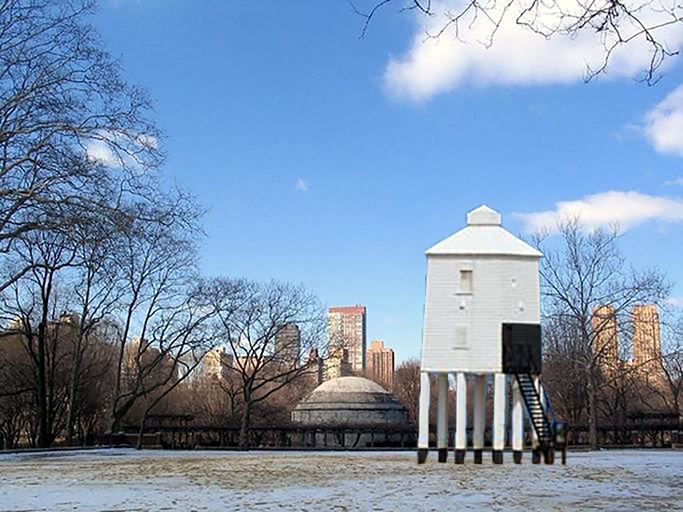
\includegraphics[width=0.7\linewidth]{figures/applications/2d_compositing.jpg}
\caption[2D compositing example]{The water tower from fig.~\ref{fig:applications_retrieval} pasted onto an image with an automatically detected similar horizon line. Note how the perspective looks right without modification.\vspace{-0.7em}}
\label{fig:applications_2d_compositing}
\vspace{-0.5em}
\end{figure}

%\vspace{-1.3em}
\paragraph{Virtual object insertion}

\newcommand{\voiwidth}{0.47}
\begin{figure}
\centering
\begin{tabular}{@{}cc@{}}
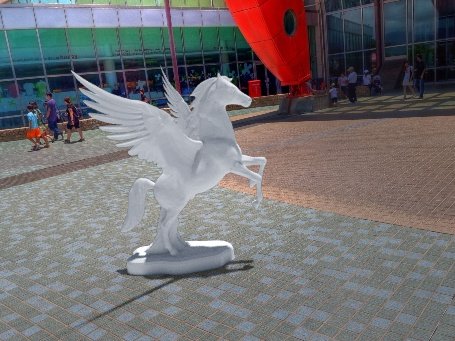
\includegraphics[width=\voiwidth\linewidth]{figures/applications/virtual_object_insertions/pano_abpaafvavryivl_jpg-2_1_es.png} &
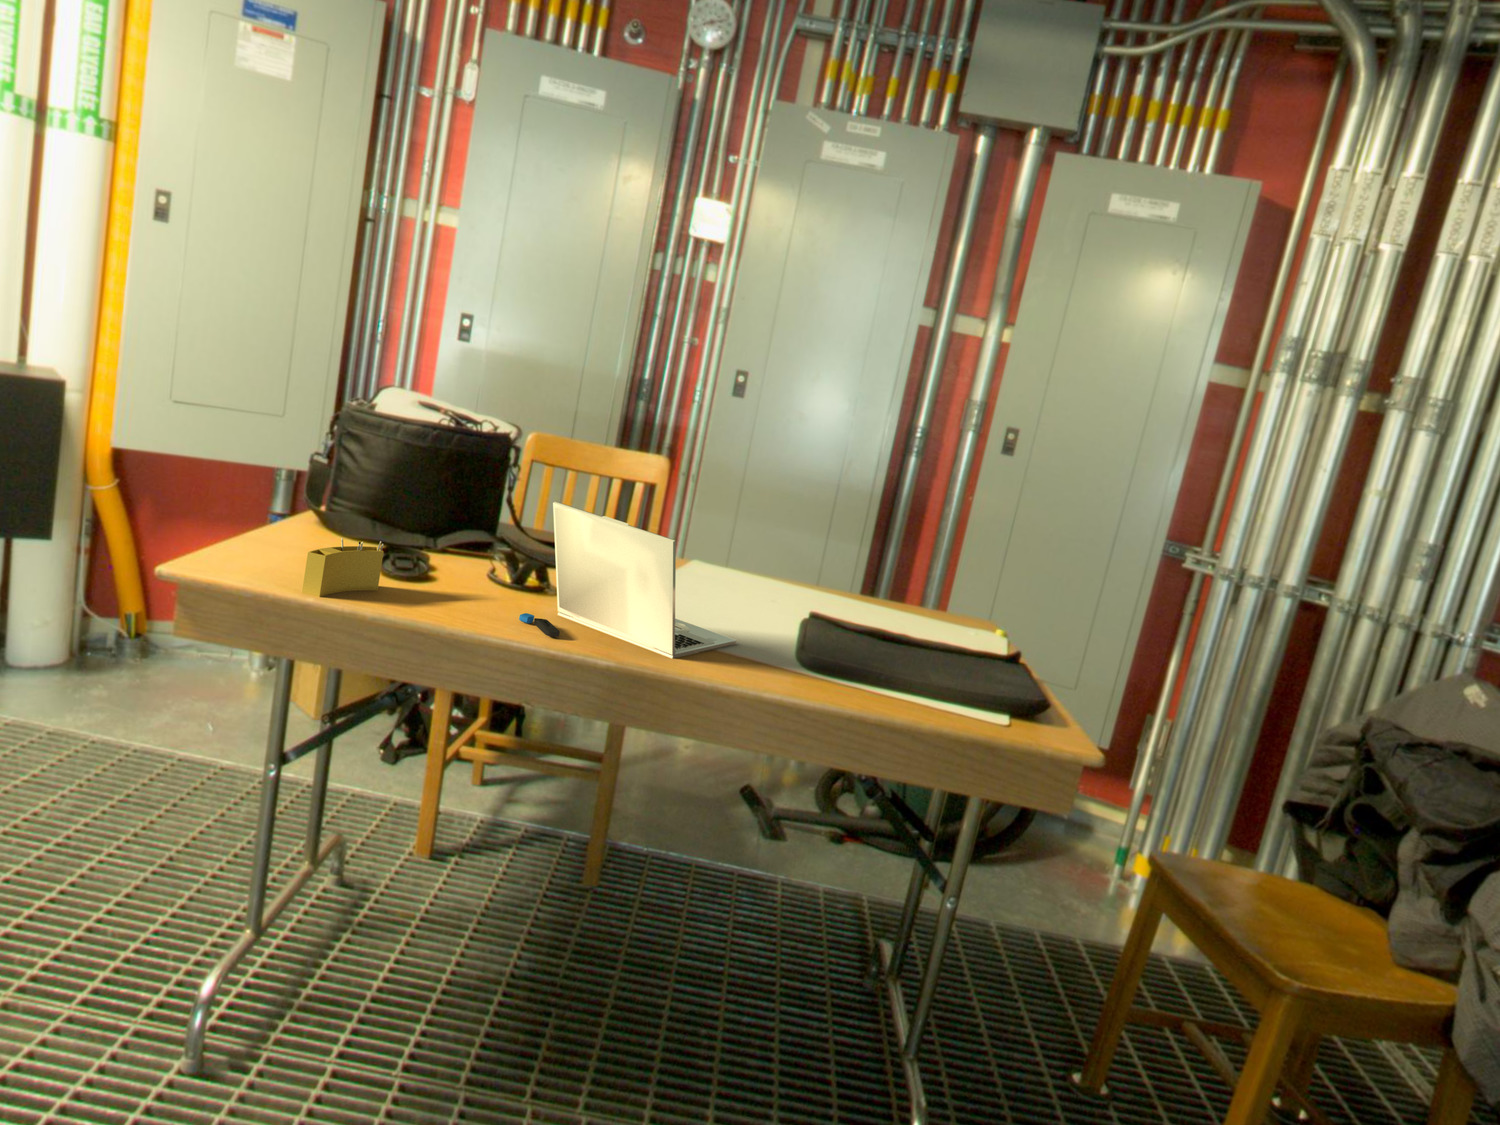
\includegraphics[width=\voiwidth\linewidth]{figures/applications/virtual_object_insertions/scene13_compose.jpg} \\
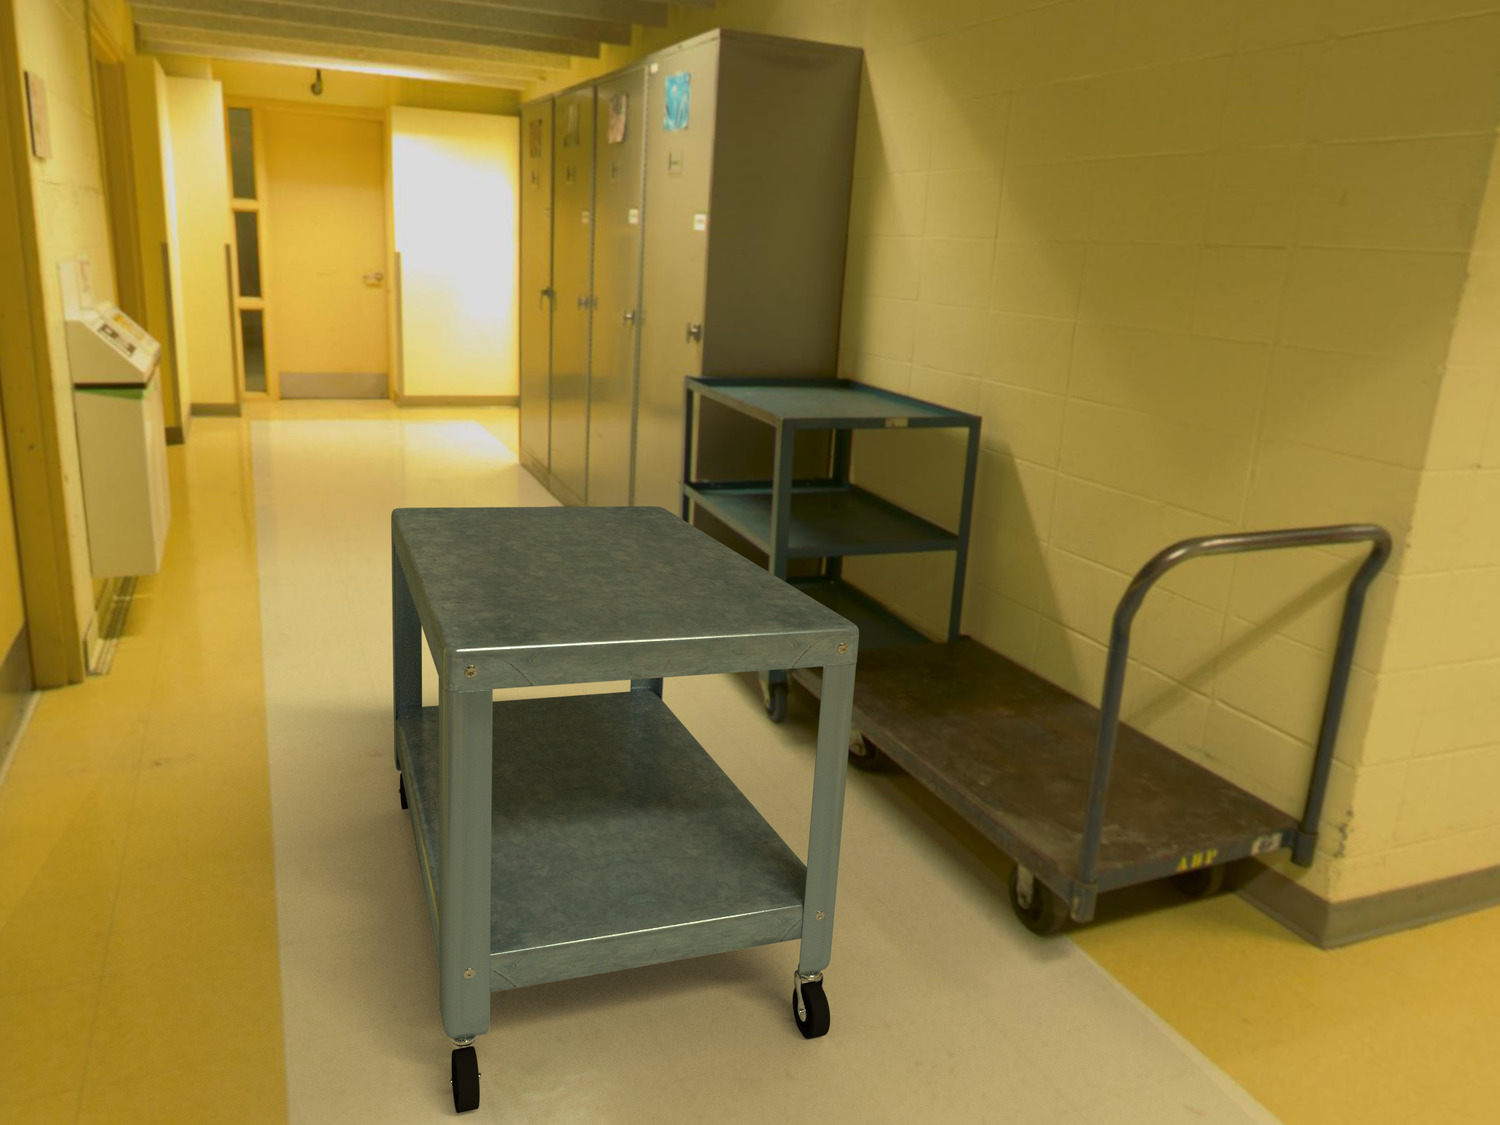
\includegraphics[width=\voiwidth\linewidth]{figures/applications/virtual_object_insertions/scene134_compose.jpg} &
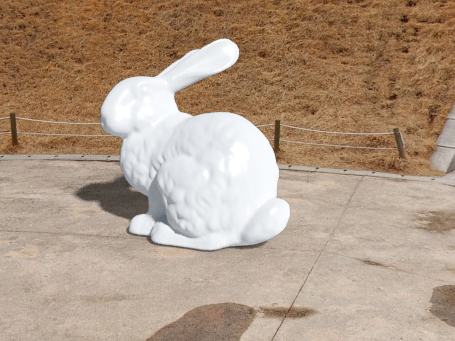
\includegraphics[width=\voiwidth\linewidth]{figures/applications/virtual_object_insertions/pano_abpebgbgmpccye_jpg-6_5_es.png}
%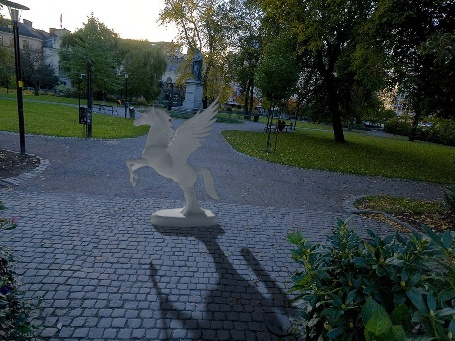
\includegraphics[height=\voiwidth\linewidth]{figures/applications/virtual_object_insertions/pano_abpezaevuxprln_jpg-0_1_es.png}
\end{tabular}
\caption[Examples of virtual object insertion]{Examples of virtual object insertions using the camera calibration estimated by our technique. \textbf{More results available in the supplementary material.}\vspace{-0.5em}}
\label{fig:applications_virtual_object_insertion}
\end{figure}

Our approach also enables the realistic insertion of 3D objects in 2D images. As discussed in sec.~\ref{sec:human_sensitivity_analysis}, camera parameters are needed to plausibly align the virtual object with the background image. Given our automatic estimates, the user only needs to select an insertion point in the image and to specify the virtual camera height. Assuming the local scene around the object is a flat plane aligned with the horizon, we can automatically insert a virtual object and demonstrate several such examples in fig.~\ref{fig:applications_virtual_object_insertion}. For these results, the camera height was set to 1.6m and the lighting was automatically estimated by~\cite{holdgeoffroy-cvpr-17,gardner-sigasia-17}.

